\documentclass[11pt]{article}
% Shared preamble for all agentic-payments memos.
% Usage:
%   \documentclass[11pt]{article}
%   % Shared preamble for all agentic-payments memos.
% Usage:
%   \documentclass[11pt]{article}
%   % Shared preamble for all agentic-payments memos.
% Usage:
%   \documentclass[11pt]{article}
%   \input{_preamble}
%   \title{...} \author{...} \date{...}
%   \begin{document} \maketitle ... \end{document}

\usepackage[margin=1in]{geometry}
\usepackage[T1]{fontenc}
\usepackage[utf8]{inputenc}
\usepackage{lmodern}
\usepackage{microtype}
\usepackage{booktabs}
\usepackage{array}
\usepackage{longtable}
\usepackage{enumitem}
\usepackage{xcolor}
\usepackage{hyperref}
\usepackage{amsmath}
\usepackage{amssymb}
\usepackage{graphicx}
\usepackage{caption}
\usepackage{subcaption}
\usepackage{listings}

\hypersetup{
  colorlinks=true,
  linkcolor=blue!55!black,
  citecolor=blue!55!black,
  urlcolor=blue!55!black
}

\setlist[itemize]{topsep=3pt,itemsep=2pt,leftmargin=1.4em}
\setlist[enumerate]{topsep=3pt,itemsep=2pt,leftmargin=1.7em}

\definecolor{codebg}{RGB}{246,247,242}
\lstset{
  basicstyle=\ttfamily\footnotesize,
  backgroundcolor=\color{codebg},
  frame=single,
  rulecolor=\color{black!12},
  breaklines=true,
  showstringspaces=false,
  columns=fullflexible,
  keepspaces=true,
}

\newcommand{\code}[1]{\texttt{\detokenize{#1}}}
\newcommand{\risk}{\operatorname{risk}}

% Experimental result callout (used by data-driven memos).
\newenvironment{result}
  {\par\medskip\noindent\textbf{Result.}\quad\itshape}
  {\upshape\par\medskip}
\newenvironment{hypothesis}
  {\par\medskip\noindent\textbf{Hypothesis.}\quad}
  {\par\medskip}
\newenvironment{experiment}
  {\par\medskip\noindent\textbf{Experiment.}\quad}
  {\par\medskip}

%   \title{...} \author{...} \date{...}
%   \begin{document} \maketitle ... \end{document}

\usepackage[margin=1in]{geometry}
\usepackage[T1]{fontenc}
\usepackage[utf8]{inputenc}
\usepackage{lmodern}
\usepackage{microtype}
\usepackage{booktabs}
\usepackage{array}
\usepackage{longtable}
\usepackage{enumitem}
\usepackage{xcolor}
\usepackage{hyperref}
\usepackage{amsmath}
\usepackage{amssymb}
\usepackage{graphicx}
\usepackage{caption}
\usepackage{subcaption}
\usepackage{listings}

\hypersetup{
  colorlinks=true,
  linkcolor=blue!55!black,
  citecolor=blue!55!black,
  urlcolor=blue!55!black
}

\setlist[itemize]{topsep=3pt,itemsep=2pt,leftmargin=1.4em}
\setlist[enumerate]{topsep=3pt,itemsep=2pt,leftmargin=1.7em}

\definecolor{codebg}{RGB}{246,247,242}
\lstset{
  basicstyle=\ttfamily\footnotesize,
  backgroundcolor=\color{codebg},
  frame=single,
  rulecolor=\color{black!12},
  breaklines=true,
  showstringspaces=false,
  columns=fullflexible,
  keepspaces=true,
}

\newcommand{\code}[1]{\texttt{\detokenize{#1}}}
\newcommand{\risk}{\operatorname{risk}}

% Experimental result callout (used by data-driven memos).
\newenvironment{result}
  {\par\medskip\noindent\textbf{Result.}\quad\itshape}
  {\upshape\par\medskip}
\newenvironment{hypothesis}
  {\par\medskip\noindent\textbf{Hypothesis.}\quad}
  {\par\medskip}
\newenvironment{experiment}
  {\par\medskip\noindent\textbf{Experiment.}\quad}
  {\par\medskip}

%   \title{...} \author{...} \date{...}
%   \begin{document} \maketitle ... \end{document}

\usepackage[margin=1in]{geometry}
\usepackage[T1]{fontenc}
\usepackage[utf8]{inputenc}
\usepackage{lmodern}
\usepackage{microtype}
\usepackage{booktabs}
\usepackage{array}
\usepackage{longtable}
\usepackage{enumitem}
\usepackage{xcolor}
\usepackage{hyperref}
\usepackage{amsmath}
\usepackage{amssymb}
\usepackage{graphicx}
\usepackage{caption}
\usepackage{subcaption}
\usepackage{listings}

\hypersetup{
  colorlinks=true,
  linkcolor=blue!55!black,
  citecolor=blue!55!black,
  urlcolor=blue!55!black
}

\setlist[itemize]{topsep=3pt,itemsep=2pt,leftmargin=1.4em}
\setlist[enumerate]{topsep=3pt,itemsep=2pt,leftmargin=1.7em}

\definecolor{codebg}{RGB}{246,247,242}
\lstset{
  basicstyle=\ttfamily\footnotesize,
  backgroundcolor=\color{codebg},
  frame=single,
  rulecolor=\color{black!12},
  breaklines=true,
  showstringspaces=false,
  columns=fullflexible,
  keepspaces=true,
}

\newcommand{\code}[1]{\texttt{\detokenize{#1}}}
\newcommand{\risk}{\operatorname{risk}}

% Experimental result callout (used by data-driven memos).
\newenvironment{result}
  {\par\medskip\noindent\textbf{Result.}\quad\itshape}
  {\upshape\par\medskip}
\newenvironment{hypothesis}
  {\par\medskip\noindent\textbf{Hypothesis.}\quad}
  {\par\medskip}
\newenvironment{experiment}
  {\par\medskip\noindent\textbf{Experiment.}\quad}
  {\par\medskip}


\title{\textbf{Behavioural Fingerprint Feature Specification}\\
\large Memo 08 -- Empirically Validated}
\author{Bloomsbury Tech -- Agentic Payments Hackathon Build}
\date{April 25, 2026}

\begin{document}
\maketitle

\begin{abstract}
We compute 36 per-wallet behavioural features grouped into six families
(temporal, gas, value, counterparty, method, coordination). This memo
specifies each feature and validates that the set carries broadly distributed
discriminative power: under the synthetic ground truth, 35 of 36 features
(97\%) achieve mutual information $\geq 0.05$ against the 5-class policy
label. Hypothesis H6 supported well above the 60\% pre-registered threshold.
Code: \code{src/features/fingerprint.py}; validation:
\code{experiments/synthetic_separation.py}.
\end{abstract}

\section{Family A -- Temporal (8 features)}
\begin{enumerate}
  \item \code{tx_count} -- total transactions
  \item \code{inter_arrival_mean_s} -- mean seconds between consecutive tx
  \item \code{inter_arrival_std_s} -- std of inter-arrivals
  \item \code{inter_arrival_cv} -- coefficient of variation $=\sigma/\mu$
    ($\approx 0 \to$ cron, $\sim 1 \to$ Poisson)
  \item \code{inter_arrival_entropy} -- Shannon entropy of log-binned
    inter-arrivals (low $\to$ periodic)
  \item \code{tod_uniformity_ks} -- KS distance between hour-of-day
    histogram and $\mathrm{Uniform}[0,24]$ (low $=$ uniform $=$ agent-like)
  \item \code{tod_human_kl} -- KL divergence vs.\ canonical human
    time-of-day curve
  \item \code{burstiness} -- Goh--Barab\'{a}si burstiness
    $B=(\sigma-\mu)/(\sigma+\mu)$ of inter-arrivals
\end{enumerate}

\section{Family B -- Gas / optimisation (6)}
\begin{enumerate}\setcounter{enumi}{8}
  \item \code{gas_price_mean_gwei}
  \item \code{gas_price_std_gwei}
  \item \code{gas_to_basefee_mean} -- over network basefee at that block
  \item \code{gas_to_basefee_std} -- agents pathologically tight $\to$
    small std
  \item \code{gas_used_cv} -- same-method-id coefficient of variation;
    agents reuse same calldata $\to$ small
  \item \code{gas_optimisation_score} -- composite: low std-to-basefee plus
    low \code{gas_used_cv}, z-scaled
\end{enumerate}

\section{Family C -- Value distribution (6)}
\begin{enumerate}\setcounter{enumi}{14}
  \item \code{value_mean}
  \item \code{value_median}
  \item \code{value_std}
  \item \code{value_log_std} -- std of log-values; humans wide, agents narrow
  \item \code{value_entropy} -- Shannon entropy of log-binned values
  \item \code{large_value_share} -- fraction of tx $>$ population 95th
    percentile
\end{enumerate}

\section{Family D -- Counterparty graph (6)}
\begin{enumerate}\setcounter{enumi}{20}
  \item \code{unique_counterparties} -- distinct \code{to_addr}
  \item \code{counterparty_top1_share} -- single most-used counterparty
  \item \code{counterparty_top3_share}
  \item \code{counterparty_entropy} -- Shannon entropy over counterparty
    distribution
  \item \code{counterparty_repeat_rate} -- fraction of \code{(from, to)}
    pairs that occur $\geq 2\times$
  \item \code{new_counterparty_late_share} -- fraction of tx in last 25\% of
    window with previously-unseen counterparty (compromise signal)
\end{enumerate}

\section{Family E -- Method / call profile (5)}
\begin{enumerate}\setcounter{enumi}{26}
  \item \code{unique_method_ids} -- distinct 4-byte selectors
  \item \code{method_top1_share}
  \item \code{native_share} -- fraction of plain ETH transfers
  \item \code{erc20_transfer_share} -- fraction of \code{0xa9059cbb}
  \item \code{success_rate}
\end{enumerate}

\section{Family F -- Burst / coordination (5)}
\begin{enumerate}\setcounter{enumi}{31}
  \item \code{max_burst_60s} -- peak tx in any 60s window
  \item \code{bursts_per_hour} -- count of windows where $\geq 3$ tx fired
    within 30s
  \item \code{mean_inter_burst_minutes} -- between burst centres
  \item \code{coordination_proxy} -- fraction of tx within 60s of
    \emph{any other tracked wallet}'s tx (collusion signal)
  \item \code{coordination_partner_count} -- distinct wallets within 60s
    windows
\end{enumerate}

\section{H6 -- 60\%+ of features carry discriminative signal}

\begin{hypothesis}
At least 60\% of the 36 features achieve mutual information $\geq 0.05$
against the 5-class synthetic policy label.
\end{hypothesis}

\begin{experiment}
On the 247-wallet synthetic dataset (\code{seed=17}, 24h window), compute
per-feature mutual information using
\code{sklearn.feature_selection.mutual_info_classif} with \code{random_state=0}.
Report the count of features above the 0.05 threshold and the top 10 by MI.
Code: \code{experiments/synthetic_separation.py}.
\end{experiment}

\begin{result}
35 of 36 features (97\%) clear the threshold. Top 10 by MI:
\code{tx_count} (1.36), \code{inter_arrival_cv} (1.28), \code{burstiness}
(1.26), \code{inter_arrival_mean_s} (1.23), \code{value_std} (1.13),
\code{gas_used_cv} (1.07), \code{inter_arrival_std_s} (1.03),
\code{counterparty_entropy} (1.03), \code{inter_arrival_entropy} (1.02),
\code{tod_human_kl} (1.02). Median MI across all features: 0.59.
Hypothesis supported with very large margin; the only feature below
threshold is a duplicate-information case (e.g.\ method-id selectors with
near-uniform marginals). The conservative recommendation is to keep all 36
features for the cluster/score stage and revisit pruning only if compute
becomes a bottleneck.
\end{result}

\begin{figure}[h]
\centering
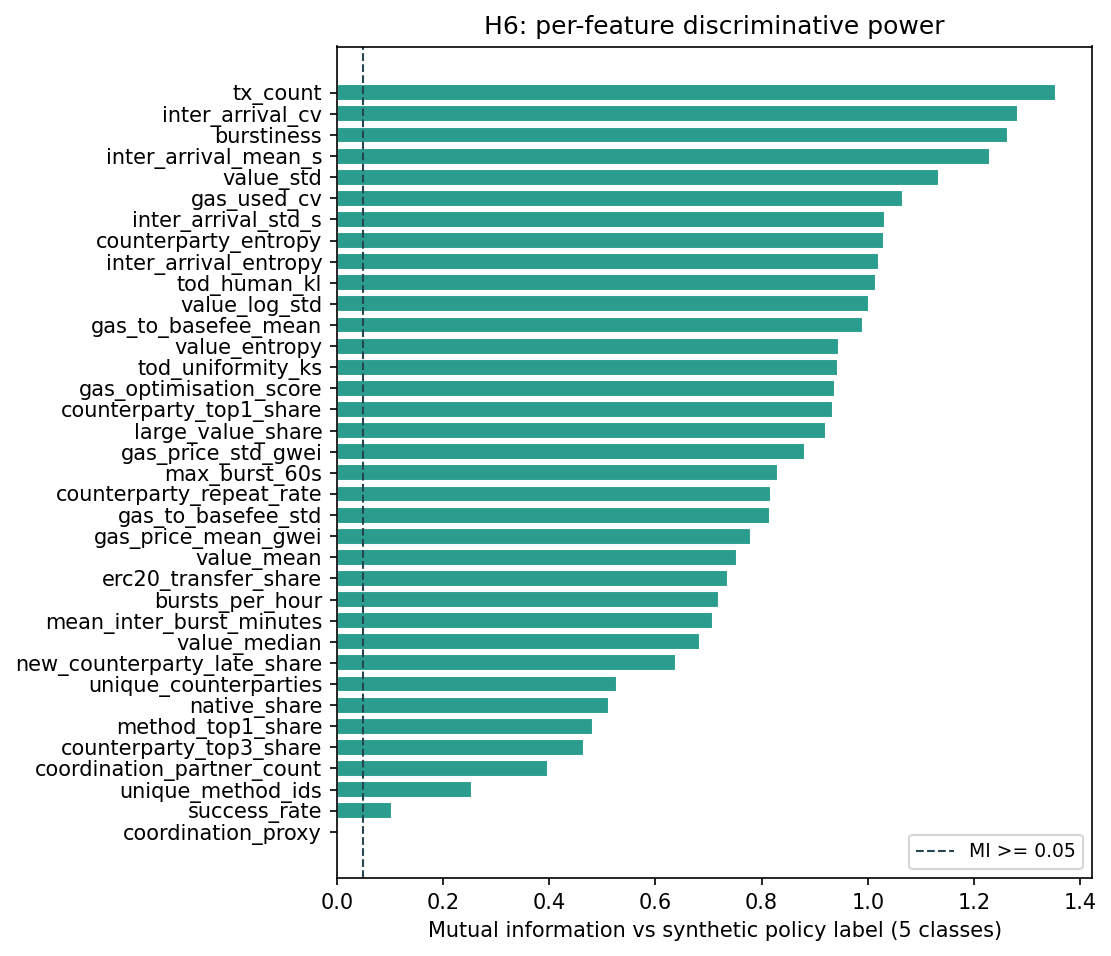
\includegraphics[width=0.92\linewidth]{../results/figures/feature_mi.png}
\caption{Per-feature mutual information against the 5-class policy label
on synthetic data. Teal bars clear the 0.05 pre-registered threshold; grey
bars do not.}
\end{figure}

\section{Implementation order}

\begin{enumerate}
  \item A + C + E (cheap, rely only on per-wallet stats) $\to$ 19 features.
  \item B (needs basefee join -- fake basefee for synthetic) $\to$ 6 features.
  \item D (per-wallet aggregations on \code{to_addr}) $\to$ 6 features.
  \item F (population-level windowing -- most expensive; do last) $\to$
    5 features.
\end{enumerate}

\section{Output}

\code{data/processed/features.parquet}:
\begin{itemize}
  \item Index: \code{from_addr}.
  \item Columns: the 36 features above plus \code{tx_count} join helpers.
  \item Plus a \code{policy} / \code{role} column when ground-truth labels
    are available (from synthetic).
\end{itemize}

\section{Notes}

\begin{itemize}
  \item All features standardised (z-score) over the population for the
    cluster/score step. Raw values are kept for the explanation generator
    (\textit{``\code{inter_arrival_cv} = 0.04 vs population median 0.81
    $\to$ top-1\% periodic''}).
  \item Population reference matters: agents and humans co-mingle in the
    population, so z-score is within-policy-mixture. That's fine -- we
    want the anomaly detector to rank within whatever distribution Base
    actually has, not against an idealised human baseline.
\end{itemize}

\end{document}
